\documentclass[document.tex]{subfiles} 
\begin{document}
\section{Аппаратное обеспечение}
\subsection{Акселерометр}
Акселерометр может применяться как для измерения проекций абсолютного линейного
ускорения, так и для косвенных~(через силу реакции опоры) измерений проекции
гравитаци\-онного ускорения.

Первое свойство используется для создания инерциальных навигационных систем, где
полученные с помощью акселерометров измерения интегрируют, получая
инерци\-альную ско\-рость и координаты носителя. Таким образом, акселерометры, наравне с
гироско\-пами, являются неотъемлемыми компонентами систем навигации и управления
самолётов, ракет и других летательных аппаратов, кораблей и подводных лодок.
Второе свойство позволяет использовать акселерометры для измерения уклонов, то
есть в качестве инклино\-метров.\cite{accelerometer_info}

Используя акселерометр в качестве инклинометра, то есть прибора,
предназначенного для измерения величины и азимута угла наклона различных
объектов относительно гравита\-ционного поля Земли, можно реализовать функционал,
характерный для уровней.

Между цифровыми и аналоговыми акселерометрами, следует выбрать цифровые, так
как они не требуют внешних компонентов, и не требуют никаких расчётов: все их
метро\-логические характеристики указаны. Стоить они будут дороже аналоговых, но
время, затра\-чиваемое на разработку системы
снижается.\cite{accelerometer_compare}

Общие сравнительные характеристики цифровых акселерометров указаны в таблице~\ref{tabular:accelerometer_compare_common}.

\begin{table}[h]
\medskip
\resizebox{\linewidth}{!}{
\tabcolsep=2pt
\begin{tabular}{|c|c|c|c|c|c|c|c|c|}
\hline
Модель&Кол-во осей&Напряжение питания&Интерфейс&
Пределы измерений&Частота выборки, Гц&Погр-ть
нуля, mg&Разрешение, mg\\
\hline
MMA7450		&3		&2.4 -- 3.6~В	&I\textsubscript{2}C, SPI	&\pm2g, \pm4g, \pm8g			&125, 250	&250	&15.6 \\
MMA7660		&3		&2.4 -- 3.6~В	&I\textsubscript{2}C		&\pm1.5g						&1 -- 120	&64		&21.33 \\
MMA7455		&3		&2.4 -- 3.6~В	&I\textsubscript{2}C, SPI	&\pm2g, \pm4g, \pm8g			&125, 250	&330	&15.6 \\
ADXL345		&3		&2.0 -- 3.6~В	&I\textsubscript{2}C, SPI	&\pm2g, \pm4g, \pm8g, \pm16g	&0.1 -- 3200&150	&3.9 \\
SMB380		&3		&2.4 -- 3.6~В	&I\textsubscript{2}C, SPI	&\pm2g, \pm4g, \pm8g			&25 -- 1500	&60		&4 \\
LIS202DL	&2		&2.2 -- 3.6~В	&I\textsubscript{2}C, SPI	&\pm2g, \pm8g					&100, 400	&40		&18 \\
LSM303DLM	&3 + 3	&2.16 -- 3.6~В	&I\textsubscript{2}C		&\pm2g, \pm4g, \pm8g			&			&60		&1 \\
\hline
\end{tabular}}
\medskip
\caption{Общие характеристики цифровых акселерометров}
\label{tabular:accelerometer_compare_common}
\end{table}

\clearpage
\subsubsection{Характеристики акселерометра MMA7660}
Неплохим выбором, исходя из таблицы~\ref{tabular:accelerometer_compare_common}, является MMA7660 компании Freescale Semiconductor, имеющий следующие технические характеристики:
\begin{itemize}
	\item цифровой вывод (I\textsubscript{2}C);
	\item 3mm x 3mm x 0.9mm DFN-чип; 
	\item низкое энергопотребление;
	\item настраиваемую частоту снятия показаний от 1 до 120 в секунду;
	\item низкий вольтаж (2.4 В -- 3.6 В~--- аналоговый; 1.71 В -- 3.6 В~--- цифровой);
	\item автоматический режим сна для уменьшения энергопотребления;
	\item определение ориентации в пространстве;
	\item совместимость с RoHS;
	\item отсутствие галогенов;
	\item низкую цену.
\end{itemize}

\noindent
Примеры типового применения акселерометра MMA7660, согласно документации, следующие:
\begin{itemize} 
	\item мобильные телефоны/ PMP/PDA: оперделение ориентации (портретная/пейзажная), стабилизация изображения, прокрутка текста, звонок по встряхиванию;
	\item настольные компьютеры: защита от кражи;
	\item игры: определение движения, автоматический режим сна для уменьшения энерго\-потребления;
	\item цифровые камеры: стабилизация изображения. \cite{accelerometer_mma7660}
\end{itemize}

\clearpage
\subsubsection{Устройство акселерометра MMA7660}
Цоколевка и функциональное устройство акселерометра MMA7660 представлены на ри\-сунке~\ref{fig:mma7660fc_pinout_scheme}.

\begin{figure}[here]
\centering
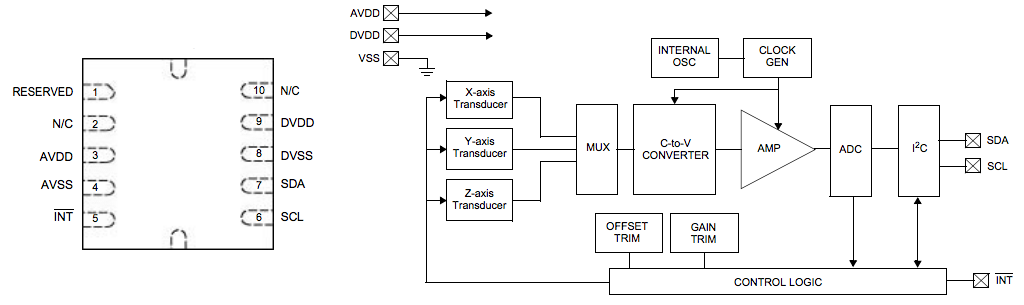
\includegraphics[width=1\linewidth]{mma7660fc_pinout_scheme}
\caption{Цоколевка и функциональное устройство акселерометра MMA7660}
\label{fig:mma7660fc_pinout_scheme}
\end{figure}

В таблице~\ref{tabular:mma7660fc_scheme} представлено описание выходов и выходов акселерометра MMA7660FC. 

\begin{table}[h]
\medskip
\resizebox{\linewidth}{!}{
\tabcolsep=2pt
\begin{tabular}{|c|c|c|c|c|c|c|c|c|}
\hline
Номер ножки&Наименование&Описание&Статус \\
\hline
1 	&RESERVED 	&Подключается к AVSS											&Вход \\
2 	&N/C 		&Без соединения, подключается к заземлению						&Вход \\
3 	&AVDD 		&Питание устройства												&Вход \\
4 	&AVSS 		&Заземление устройства											&Вход \\
5 	&INT 		&Прерывание/готовность данных									&Выход \\
6 	&SCL 		&Тактовые импульсы I\textsubscript{2}C 							&Вход \\
7 	&SDA 		&Последовательные данные I\textsubscript{2}C					&Открытый коллектор \\
8 	&DVSS 		&Цифровое заземление I/O										&Вход \\
9 	&DVDD 		&Цифровое питание I/O											&Вход \\
10 	&N/C 		&Без соединения, подключается к заземлению						&Вход \\
\hline
\end{tabular}}
\medskip
\caption{Общие характеристики цифровых акселерометров}
\label{tabular:mma7660fc_scheme}
\end{table}

\clearpage
\subsubsection{Подключение акселерометра MMA7660 к микроконтроллеру}
Акселерометр MMA7660 подключается к микроконтроллеру с использованием протокола I\textsubscript{2}C. Схема подключения представлена на рисунке~\ref{fig:mma7660fc_connection}.

\begin{figure}[here]
\centering
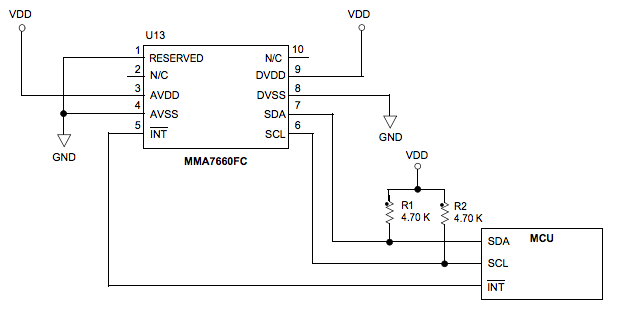
\includegraphics[width=0.7\linewidth]{mma7660fc_connection}
\caption{Цоколевка и функциональное устройство акселерометра MMA7660}
\label{fig:mma7660fc_connection}
\end{figure}

Входы AVDD и DVDD подключаются к источнику питания, входы AVSS и DVSS (опцио\-нально, входы N/C) подключаются к заземлению, выход INT подключается к микрокон\-троллеру
напрямую, а контакты SCL и SDA из-за использования открытых коллекторов, подключаются с использованием подтягивающих резисторов на 4.7 кОм.

\clearpage
\subsubsection{Тайминги акселерометра MMA7660}
На рисунке~\ref{fig:mma7660fc_timing_common} показан общий тайминг протокола I\textsubscript{2}C, используемого акселерометром для передачи и приема данных с микроконтроллера.
\begin{figure}[here]
\centering
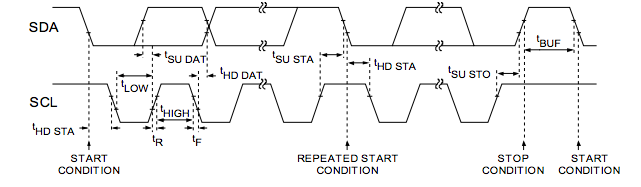
\includegraphics[width=0.8\linewidth]{mma7660fc_timing_common}
\caption{Общий тайминг протокола I\textsubscript{2}C акселерометра MMA7660}
\label{fig:mma7660fc_timing_common}
\end{figure}

\end{document}
